
\documentclass[%
 reprint,
%superscriptaddress,
%groupedaddress,
%unsortedaddress,
%runinaddress,
%frontmatterverbose, 
%preprint,
%preprintnumbers,
nofootinbib,
%nobibnotes,
%bibnotes,
 amsmath,amssymb,
 aps,
%pra,
%prb,
%rmp,
%prstab,
%prstper,
floatfix,
]{revtex4-2}
\usepackage{gensymb}
\usepackage{textcomp}
\usepackage{lipsum}
\usepackage{graphicx}% Include figure files
\usepackage{dcolumn}% Align table columns on decimal point 


\usepackage{bm}% bold math
\usepackage{siunitx}
\DeclareSIUnit\gauss{G}
\DeclareSIUnit\erg{erg}
\DeclareMathOperator{\Rot}{rot}
\sisetup{separate-uncertainty=true}
\usepackage{tabularx}
\usepackage{amssymb}
\usepackage{amsmath}
\usepackage{relsize}
\usepackage{commath}
\usepackage{enumitem}
\usepackage{xfrac}
\usepackage{float}
\usepackage{booktabs}
\usepackage{makecell}
\usepackage{caption}
\usepackage{longtable}
\usepackage{bm}
\usepackage{subcaption}
\usepackage{breqn}
\DeclareSIUnit{\angstrom}{\textup{\AA}}
\usepackage{multirow}
\usepackage[version=4]{mhchem}
\usepackage[colorlinks,bookmarks=false,citecolor=blue,linkcolor=blue,urlcolor=blue]{hyperref}
%\usepackage{hyperref}% add hypertext capabilities
%\usepackage[mathlines]{lineno}% Enable numbering of text and display math
%\linenumbers\relax % Commence numbering lines

%\usepackage[showframe,%Uncomment any one of the following lines to test 
%%scale=0.7, marginratio={1:1, 2:3}, ignoreall,% default settings
%%text={7in,10in},centering,
%%margin=1.5in,
%%total={6.5in,8.75in}, top=1.2in, left=0.9in, includefoot,
%%height=10in,a5paper,hmargin={3cm,0.8in},
%]{geometry}

\begin{document}

\preprint{APS/123-QED}

\title{Gamma-ray Spectroscopy}% Force line breaks with \\


\author{Maitrey Sharma}
\email{maitrey.sharma@niser.ac.in}
\affiliation{School of Physical Sciences, National Institute of Science Education and Research, HBNI, Jatni-752050, India}




\date{\today}% It is always \today, today,
             %  but any date may be explicitly specified

\begin{abstract}
    Herein we perform the quantitative analysis of gamma energy spectrums from different radioactive sources. We understand the functioning of Single and multi channel analyzer by using them to calibrate the detector for the known Cs-137 source. We also perform the analysis on multipeak source such as Co-60 and on a mixed sample (containing 3 different radioactive substances). We also found the unknown radioactive material from its spectrum which was found to be Na-22. Finally, we also looked at the effects of absorber on the gamma rays and determined the mass absorption coefficient of Aluminium.
\end{abstract}

\keywords{}
\maketitle

%\tableofcontents


    
\section{Aim}
    Our primary objectives in this experiment are
    \begin{enumerate}
        \item Using Single Channel Analyzer (SCA), study the dependence of energy resolution on the applied voltage and to determine the best Operating Voltage for the Scintillation Detector.
        \item Using Multi Channel Analyzer (MCA), study the Cs-137 spectrum and calculate the FWHM and find the resolution for the Scintillation Detector.
        \item Using MCA, study of Co-60 Spectrum and Calculation of resolution of the detector in terms of energy.
        \item Using MCA, callibrate gamma ray spectrometer (linearity study) by Manual Calculation method.
        \item Using MCA, determine the unknown energy of a radioactive isotope.
        \item Using MCA, find the mass absorption coefficient of Aluminium.
    \end{enumerate}
    
\section{Apparatus}
    The apparatus used in this experiment are
    \begin{enumerate}
        \item Scintillation detector apparatus
        \item Amplifier with ADC
        \item Cs-137 source
        \item Aluminium plate
        \item MCA
        \item Anuspect Software
        \item Different Radioactive Source
    \end{enumerate}



\section{Theory}
\subsection{Photomultiplier Tube}
In a PMT, when radiation is incident on the scintillation detector, it falls on the crystal NaI (activated by Thallium); which leads to ionization creating excited states in the crystal, that further decays by photons. Thallium is required to activate as it protects the photo cathode material by shifting the wavelength of those photons to which it is sensitive to. The crystal is optically coupled to photocathode, which is followed by a series of plates called dynodes. The incident scintillated photons falling on the photocathode releases photoelectrons which then gets amplified by the series of dynodes. This happens because the dynode arrangement is in such a way that the electrons sees each of them at a higher positive voltage than the previous one. Hence they get accelerated towards each dynode and each strike emits more and more electrons. This whole setup from
photo-cathode to anode is known as photo-multiplier tube(PMT).\\

\subsection{Multi Channel Analyzer (MCA)}
 The MCA is based on ADC (analog to digital converter) technique where a built in periodic oscillation sends out clock pulses. The output of the ADC (the number of clock pulses in that time interval) is stored in computer memory. The spectra obtained in such a way is subdivided into addressable channels whose number is in power of two. In order to find out which channel number corresponds to which energy, we need to do energy calibration, which is obtained by using radioactive sources which emit gamma quanta with known energies.
 
 In the last part of the experiment we are calculating the mass absorption coefficient of Aluminium from Lambert’s law. The law states that the decrease of intensity of radiation as it passes through an absorber is given by:
 \begin{equation}
     I = I_0 \exp{-mx}
 \end{equation}
where, \\
I = intensity after the absorber\\
I0 = intensity before the absorber\\
m = total mass absorption coefficient in cm2/g\\
x = density thickness in g/cm2\\

\subsection{Gamma Ray Spectrometer}
We get a whole spectrum of energies at the output as the total charge getting accumulated at
anode is proportional to the energy deposited by the
incident radiation in the detector. The pre-amplifier converts anode charges to a voltage pulse. The Gamma Ray Spectrometer consist of High Volt-age Unit, linear amplifier, single channel analyzer(SCA) and a counter timer. The linear amplifier amplifies
the signal received from pre-amplifer and also performs
pulse shaping. Counter timer is used in counting the
number of events in a preset time. The SCA helps to get information about the incident radiation by counting the pulses along with the energy and timing information. The module generates a logic pulse only when the input voltage
height lies in between a certain limit. The entire voltage input is chopped into bins of voltages by selecting lower and upper limits as the voltage pulse is proportional to the energy. These limits are known as Lower Level Discrimination (LLD) and
Upper Level Discrimination (ULD). Resolution of a scintillation spectrometer is defined as the ’full-width at half max-
imum of the photo-peak spectrum.\\ 

\textbf{FWHM:} Full width at half maximum is the channel width of the CS- 137 photo-peak spectrum at hall the peak height. In the graph of photo-peak spectrum, one can draw a horizontal line at half peak height and see the width. \\

\textbf{Resolution:} Resolution of a NaI scintillation detector is defined as the ratio of FWHM divided by peak channel LLD value.
$$
\text { Resolution }=\left(\dfrac{\text{FWHM}}{\text{peak channel LLD value}}\right) \times 100
$$

Both resolution \& FWHM are important for NaI scintillation detectors and are universally specified with a Cs-137 standard source by the manufacturer of the detector when they supply. Typically resolution for these detectors range from $7.5 \%$ to $9.5 \%$.

 Gamma Ray Spectrometer GR611M (Modular Minim based) is shown in Fig 1.
\begin{figure}[H]
    \centering
    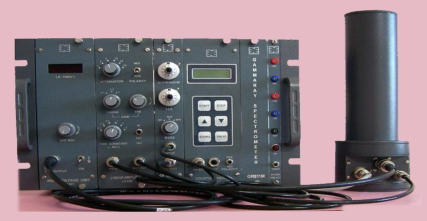
\includegraphics[angle=0,width=10cm]{Figures/spectrometer.png}
    \caption{Gamma Ray Spectrometer GR611M}
    \label{Table.1.}
\end{figure}

\section{Observations and Evaluation}
\subsection{Single Channel Analyzer (Part A)}
We set the LLD (lower-level discrimination) in the first part from 2.5 V to 3.6 V with ULD (upper-level discrimination) set at 0.1 V higher than LLD. The preset time was set as 30s. Counts were recorded for different operating voltages.

\begin{table*}[]
\caption{Readings for the SCA part of the experiment}
\label{tab:my-table}
\begin{tabular}{@{}ccccccccccccccccc@{}}
\toprule
\multicolumn{2}{c}{\textbf{450   V}} &  & \multicolumn{2}{c}{\textbf{450 V}} &  & \multicolumn{2}{c}{\textbf{550 V}} &  & \multicolumn{2}{c}{\textbf{600 V}} &  & \multicolumn{2}{c}{\textbf{650 V}} &  & \multicolumn{2}{c}{\textbf{700 V}} \\ \cmidrule(r){1-2} \cmidrule(lr){4-5} \cmidrule(lr){7-8} \cmidrule(lr){10-11} \cmidrule(lr){13-14} \cmidrule(l){16-17} 
\textbf{Base Line} & \textbf{Counts} &  & \textbf{Base Line} & \textbf{Counts} &  & \textbf{Base Line} & \textbf{Counts} &  & \textbf{Base Line} & \textbf{Counts} &  & \textbf{Base Line} & \textbf{Counts} &  & \textbf{Base Line} & \textbf{Counts} \\ \midrule
2.5 & 639 &  & 2.4 & 693 &  & 2.4 & 1039 &  &  &  &  &  &  &  &  &  \\
2.6 & 697 &  & 2.5 & 736 &  & 2.5 & 803 &  & 2.5 & 2080 &  & 2.5 & 3764 &  & 2.5 & 2304 \\
2.7 & 1049 &  & 2.6 & 1225 &  & 2.6 & 694 &  & 2.6 & 2143 &  & 2.6 & 7107 &  & 2.6 & 4549 \\
2.8 & 2204 &  & 2.7 & 2589 &  & 2.7 & 775 &  & 2.7 & 2559 &  & 2.7 & 10477 &  & 2.7 & 8314 \\
2.9 & 4484 &  & 2.8 & 5207 &  & 2.8 & 1267 &  & 2.8 & 3132 &  & 2.8 & 8257 &  & 2.8 & 8578 \\
3 & 7824 &  & 2.9 & 8730 &  & 2.9 & 2633 &  & 2.9 & 5221 &  & 2.9 & 6780 &  & 2.9 & 7086 \\
3.1 & 9412 &  & 3 & 9374 &  & 3 & 5043 &  & 3 & 8865 &  & 3 & 5734 &  & 3 & 5924 \\
3.2 & 6912 &  & 3.1 & 5851 &  & 3.1 & 8216 &  & 3.1 & 7148 &  & 3.1 & 4919 &  & 3.1 & 5571 \\
3.3 & 2902 &  & 3.2 & 2275 &  & 3.2 & 8885 &  & 3.2 & 5511 &  & 3.2 & 4207 &  & 3.2 & 4885 \\
3.4 & 1028 &  & 3.3 & 788 &  & 3.3 & 5559 &  & 3.3 & 4424 &  & 3.3 & 3594 &  & 3.3 & 4623 \\
3.5 & 413 &  & 3.4 & 372 &  & 3.4 & 2333 &  & 3.4 & 3302 &  & 3.4 & 3034 &  & 3.4 & 4344 \\
 &  &  &  &  &  & 3.5 & 749 &  & 3.5 & 2547 &  & 3.5 & 2463 &  & 3.5 & 3805 \\
 &  &  &  &  &  & 3.6 & 420 &  &  &  &  &  &  &  &  &  \\ \bottomrule
\end{tabular}
\end{table*}

\begin{figure}[H]
    \centering
    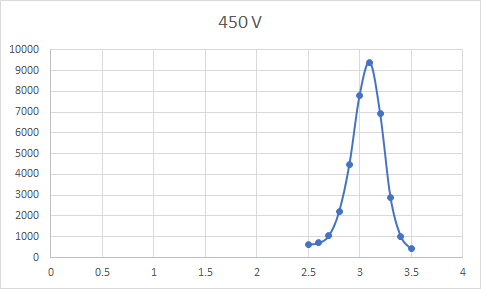
\includegraphics[width = 8 cm]{Figures/450.png}
    \caption{SCA plot for 450 V}
    \label{fig:my_label}
\end{figure}
\begin{itemize}
    \item The peak is found at the base voltage = 3.2 V.
    \item The FWHM of the observed graph = 0.36 V.
    \item The resolution is found to be = 11.25 \%.
\end{itemize}
\begin{align*}
    \centering \textbf{Operating Voltage = 500 V}
\end{align*}

% Please add the following required packages to your document preamble:
% \usepackage{longtable}
% Note: It may be necessary to compile the document several times to get a multi-page table to line up properly


\begin{figure}[H]
    \centering
    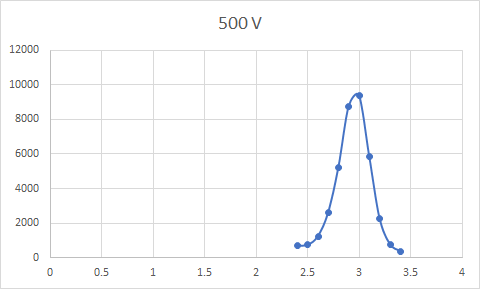
\includegraphics[width = 8 cm]{Figures/500.png}
    \caption{SCA plot for 500 V}
    \label{fig:my_label}
\end{figure}

\begin{itemize}
    \item The peak is found at the base voltage = 3.1 V.
    \item The FWHM of the observed graph = 0.37 V.
    \item The resolution is found to be = 111.935 \%.
\end{itemize}
\begin{align*}
    \centering \textbf{Operating Voltage = 550 V}
\end{align*}
% Please add the following required packages to your document preamble:
% \usepackage{longtable}
% Note: It may be necessary to compile the document several times to get a multi-page table to line up properly


\begin{figure}[H]
    \centering
    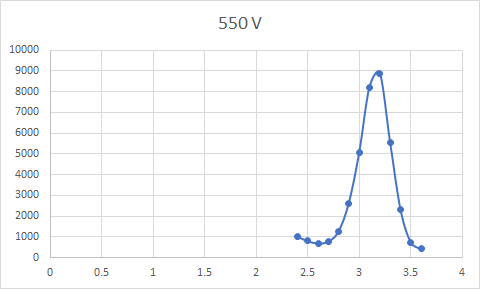
\includegraphics[width = 8 cm]{Figures/550.png}
    \caption{SCA plot for 550 V}
    \label{fig:my_label}
\end{figure}

\begin{itemize}
    \item The peak is found at the base voltage = 3 V.
    \item The FWHM of the observed graph = 0.28 V.
    \item The resolution is found to be = 9.334 \%.
\end{itemize}
\begin{align*}
    \centering \textbf{Operating Voltage = 600 V}
\end{align*}
% Please add the following required packages to your document preamble:
% \usepackage{longtable}
% Note: It may be necessary to compile the document several times to get a multi-page table to line up properly


\begin{figure}[H]
    \centering
    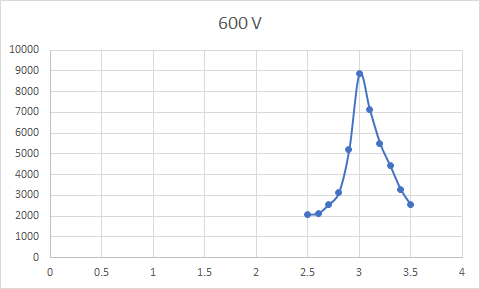
\includegraphics[width = 8 cm]{Figures/600.png}
    \caption{SCA plot for 600 V}
    \label{fig:my_label}
\end{figure}

\begin{itemize}
    \item The peak is found at the base voltage = 3 V.
    \item The FWHM of the observed graph = 0.42 V.
    \item The resolution is found to be = 14 \%.
\end{itemize}
\begin{align*}
    \centering \textbf{Operating Voltage = 650 V}
\end{align*}
% Please add the following required packages to your document preamble:
% \usepackage{longtable}
% Note: It may be necessary to compile the document several times to get a multi-page table to line up properly


\begin{figure}[H]
    \centering
    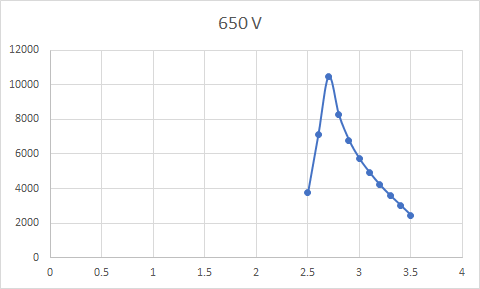
\includegraphics[width = 8 cm]{Figures/650.png}
    \caption{SCA plot for 650 V}
    \label{fig:my_label}
\end{figure}

\begin{itemize}
    \item The peak is found at the base voltage = 2.9 V.
    \item The FWHM of the observed graph = 0.57 V.
    \item The resolution is found to be = 19.655 \%.
\end{itemize}

\begin{align*}
    \centering \textbf{Operating Voltage = 700 V}
\end{align*}
\begin{figure}[H]
    \centering
    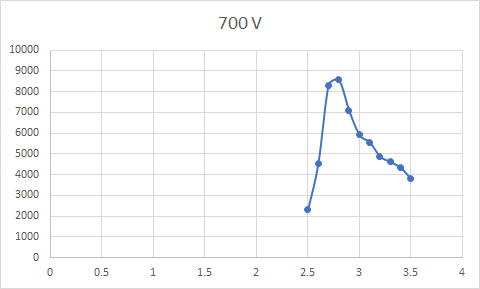
\includegraphics[width = 8 cm]{Figures/700.png}
    \caption{SCA plot for 700 V}
    \label{fig:my_label}
\end{figure}

\begin{itemize}
    \item The peak is found at the base voltage = 2.9 V.
    \item The FWHM of the observed graph = 0.57 V.
    \item The resolution is found to be = 19.655 \%.
\end{itemize}
$\implies$ We can conclude that the operating voltage for our further experiments should be chosen as 550 V as it offers the least resolution value of 9.33 $\%$ (the lower the value, better the operation).

% Please add the following required packages to your document preamble:
% \usepackage{booktabs}
\begin{table}[]
\caption{After determining the operating voltage we take the spectrum acquisition with SCA}
\label{tab:my-table}
\begin{tabular}{@{}cc@{}}
\toprule
\multicolumn{2}{c}{\textbf{550V}} \\ \midrule
\textbf{Base line} & \textbf{Counts} \\
0.5 & 3301 \\
0.6 & 3470 \\
0.7 & 3614 \\
0.8 & 3902 \\
0.9 & 4197 \\
1 & 4140 \\
1.1 & 3499 \\
1.2 & 3157 \\
1.3 & 2852 \\
1.4 & 2785 \\
1.5 & 2639 \\
1.6 & 2579 \\
1.7 & 2498 \\
1.8 & 2350 \\
1.9 & 2376 \\
2 & 2374 \\
2.1 & 2162 \\
2.2 & 1965 \\
2.3 & 1613 \\
2.4 & 1226 \\
2.5 & 913 \\
2.6 & 778 \\
2.7 & 779 \\
2.8 & 1070 \\
2.9 & 1823 \\
3 & 3720 \\
3.1 & 6877 \\
3.2 & 9010 \\
3.3 & 7241 \\
3.4 & 3905 \\
3.5 & 1384 \\
3.6 & 509 \\
3.7 & 301 \\
3.8 & 227 \\ \bottomrule
\end{tabular}
\end{table}
\begin{figure}
    \centering
    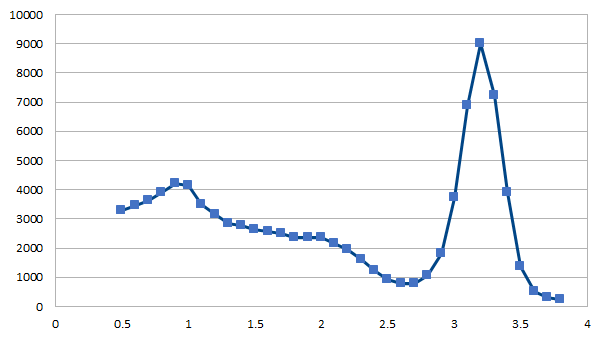
\includegraphics[scale = 0.7]{Figures/sca-cs-137.png}
    \caption{Counts with Cs-137 at operating voltage with SCA}
    \label{fig:my_label}
\end{figure}
\subsection{Multi Channel Analyzer (MCA) - Part B}
We made the use of Anuspect Software in the lab to analyze the graphs obtained by our apparatus. Further calculations is based on the reports generated by the software.
We first calibrated the channels using Cs 137 source and keeping that as the reference, plotted other spectras. 
\newpage
\subsubsection*{Study of Cs-137 Spectrum}


\begin{figure}[H]
    \centering
    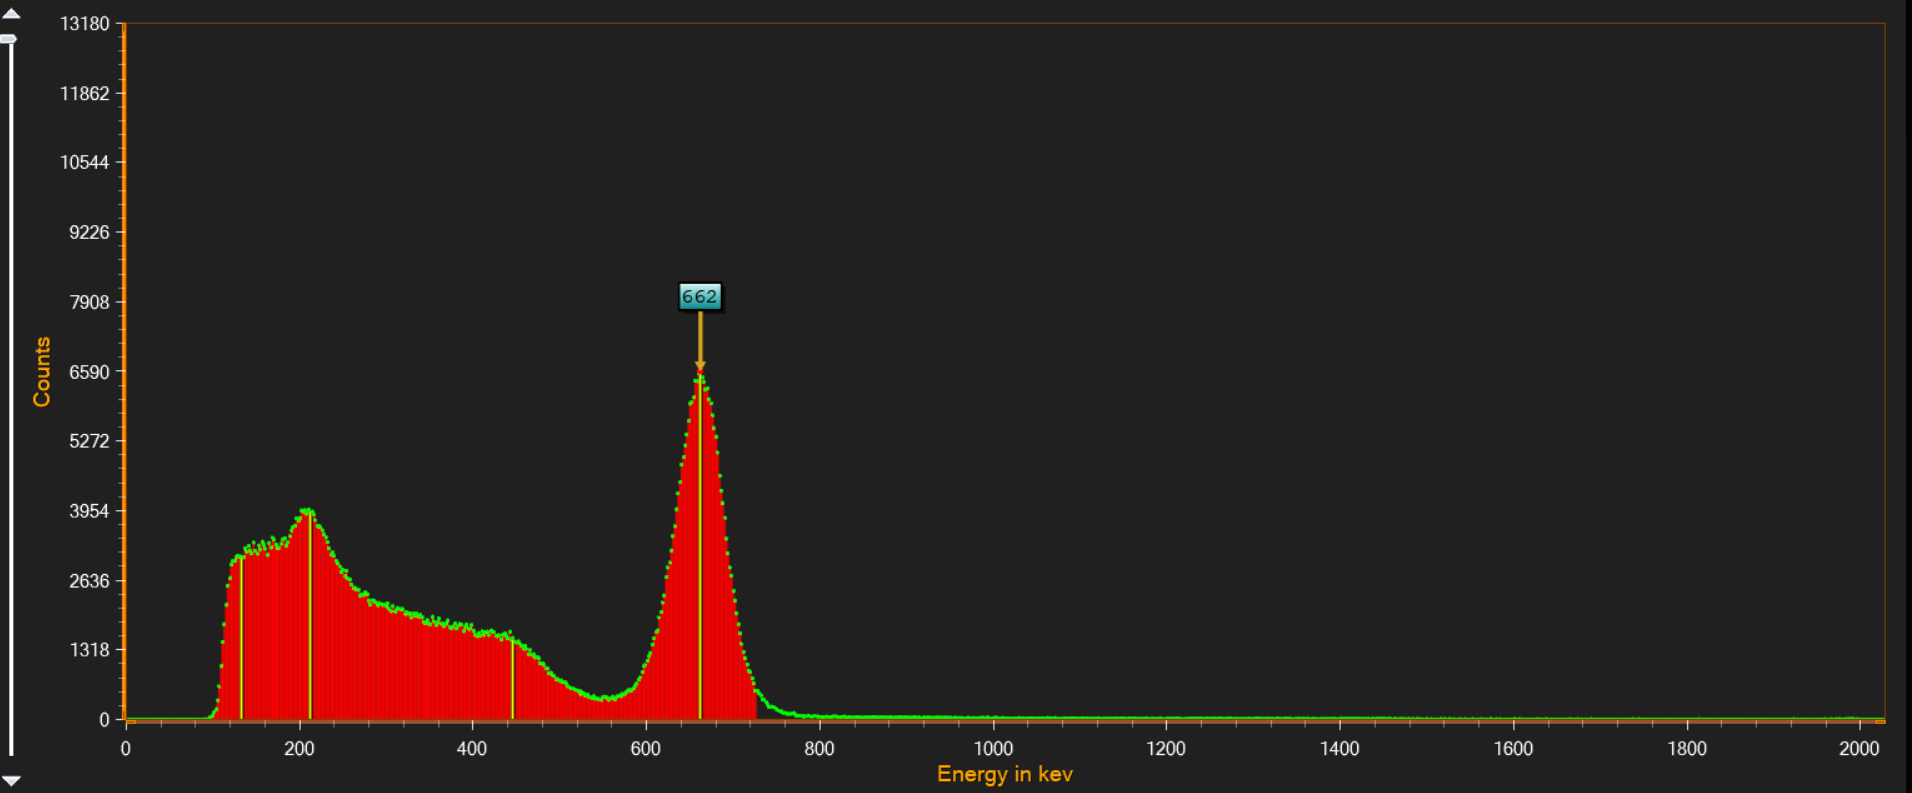
\includegraphics[width = 8 cm]{Figures/cs-137.png}
    \caption{Counts Vs Channel Number plot for Cs-137}
    \label{fig:my_label}
\end{figure}
\begin{figure}
    \centering
    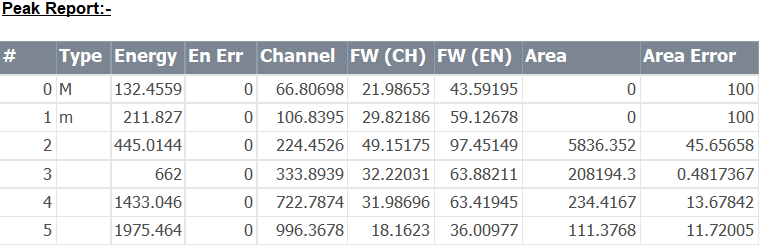
\includegraphics[scale = 0.3]{Figures/cs-137-report.PNG}
    \caption{Report generated for Cs-137}
    \label{fig:my_label}
\end{figure}
From the report generated by the software we find that:\\
\begin{itemize}
    \item FWHM channel = 29.6378
    \item FWHM Energy = 61.878 keV
    \item Peak Channel = 317.078
    \item Hence the resolution is given by:
    \begin{dmath*}
        \textit{Resolution} = \frac{FWHM}{Peak Channel} = \frac{29.6378}{317.078}
         = 9.347 \%.
    \end{dmath*}
\end{itemize}

\subsubsection*{Study of Co-60 Spectrum and Calculation of resolution of the detector in terms of energy.}
\begin{figure}[H]
    \centering
    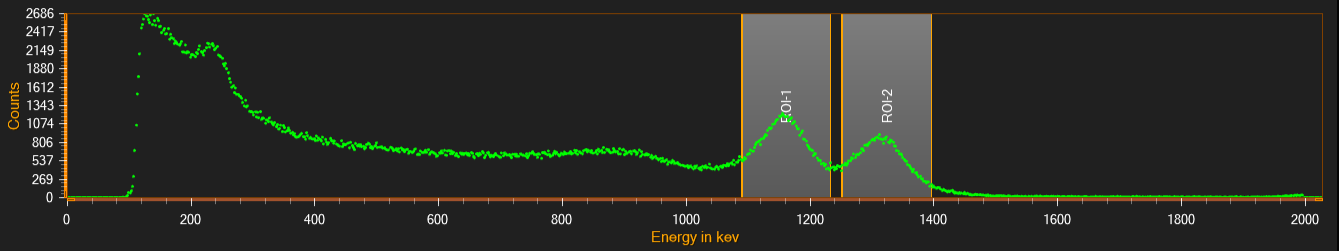
\includegraphics[width = 8 cm]{Figures/Co-60_energyspectrum.PNG}
    \caption{Counts Vs Channel Number plot for Co-60}
    \label{fig:my_label}
\end{figure}
\begin{figure}
    \centering
    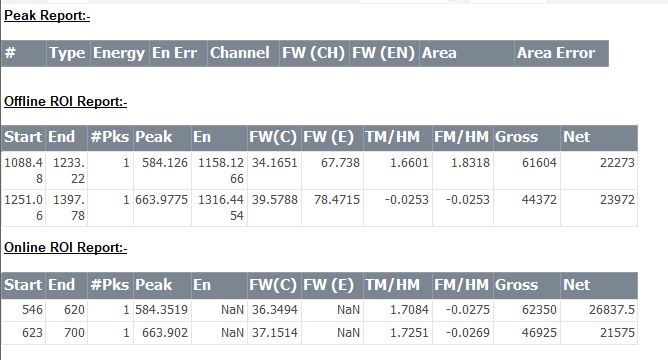
\includegraphics[scale = 0.3]{Figures/Co-60_report.PNG}
    \caption{Report generated for C0-60}
    \label{fig:my_label}
\end{figure}
\centering For the 1st peak:\\
\begin{itemize}
    \item Peak Channel Number = 557.9709
    \item Peak Energy = 1164.9391 keV
\end{itemize}

\centering For the 2nd peak:\\
\begin{itemize}
    \item Peak channel Number = 634.3788
    \item Peak Energy = 1324.4645 keV
\end{itemize}
Now we see that the two peaks' channel number difference is 76.4079 which corresponds to an energy difference of 159.5254 keV.\\
We can say that 1 channel corresponds to $\frac{159.5254}{76.4079}$ = 2.0878 KeV of energy.\\
Using the previous part of Cs calibration, we know that FWHM is 29.6378 and hence in terms of energy we get FWHM energy = 29.6378 $\times$ 2.0878 = 61.88 keV. \\
$\implies$ The resolution is given by\\
    \begin{dmath*}
        \textit{Resolution} = \frac{FWHM}{Peak Channel} = \frac{61.88}{662}
         = 9.347 \%.
    \end{dmath*}
    
\subsubsection*{Energy calibration of Gamma ray Spectrometer using MCA (linearity study)}
\begin{figure}[H]
    \centering
    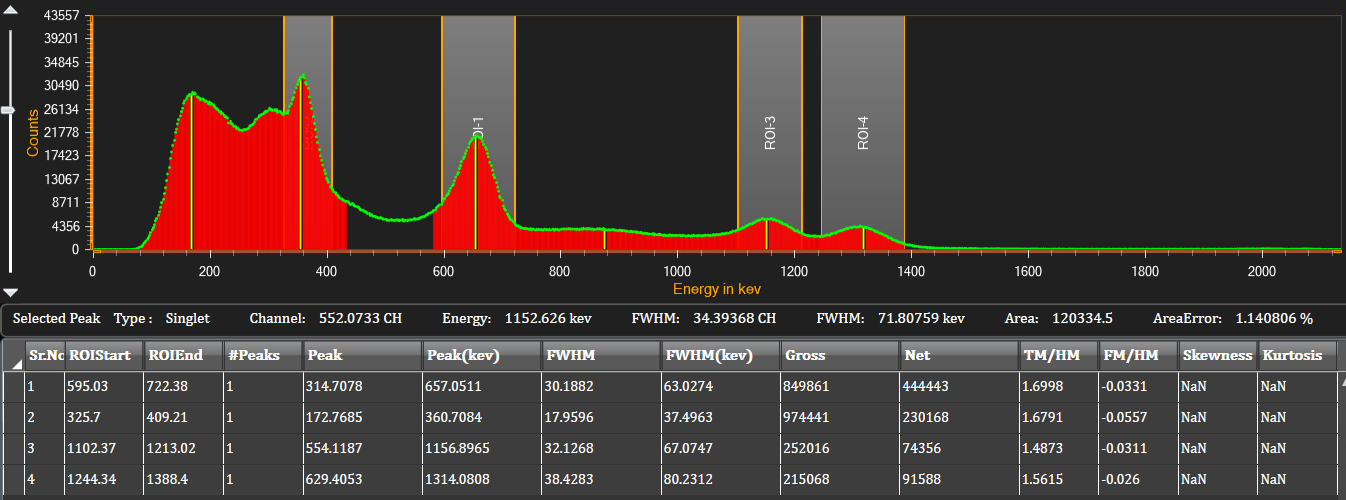
\includegraphics[width = 8 cm]{Figures/Multiple sources.png}
    \caption{Counts Vs Energy plot for 3 mixed sources}
    \label{fig:my_label}
\end{figure}
\begin{figure}
    \centering
    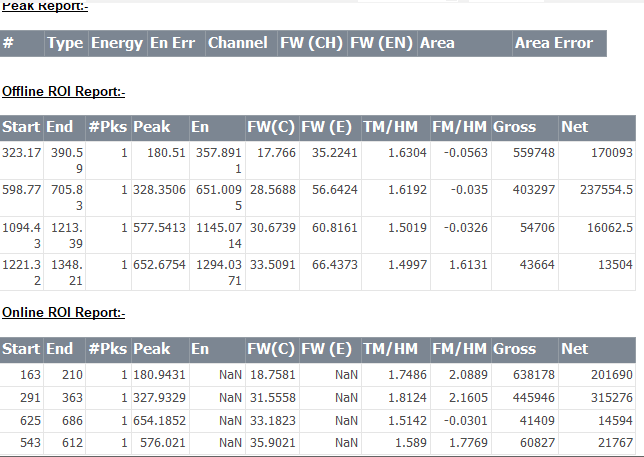
\includegraphics[scale = 0.3]{Figures/Threesources_report.PNG}
    \caption{Report generated for multiple sources}
    \label{fig:my_label}
\end{figure}
Using the observed spectra we can plot the graph between peak channel number and the corresponding energies as tabulated below:
% Please add the following required packages to your document preamble:
% \usepackage{longtable}
% Note: It may be necessary to compile the document several times to get a multi-page table to line up properly
\begin{longtable}[c]{|l|l|l|}
\hline
\textbf{Source} & \textbf{Channel} & \textbf{Energy (keV)} \\ \hline
\endfirsthead
%
\endhead
%
Ba-133 & 172.7685 & 360.7084 \\ \hline
Cs-137 & 314.7078 & 657.0511 \\ \hline
Co-60 & 554.1187 & 1156.897 \\ \hline
Co-60 & 629.4053 & 1314.081 \\ \hline
\end{longtable}
\begin{figure}[H]
    \centering
    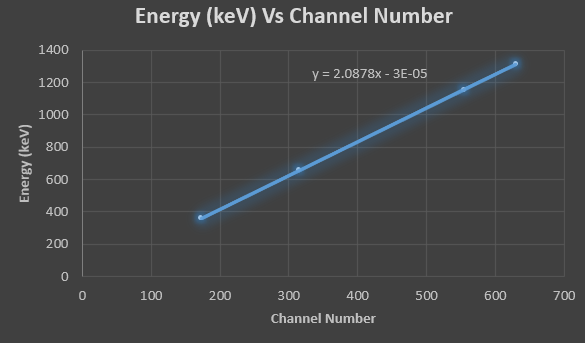
\includegraphics[width = 8 cm]{Figures/Screenshot (236).png}
    \caption{Linearity plot for multiple sources}
    \label{fig:my_label}
\end{figure}
We can identify the sources from their peak positions in graph. We also observe a linear relation as was expected.

\subsubsection*{Spectra of unknown source}
\begin{figure}[H]
    \centering
    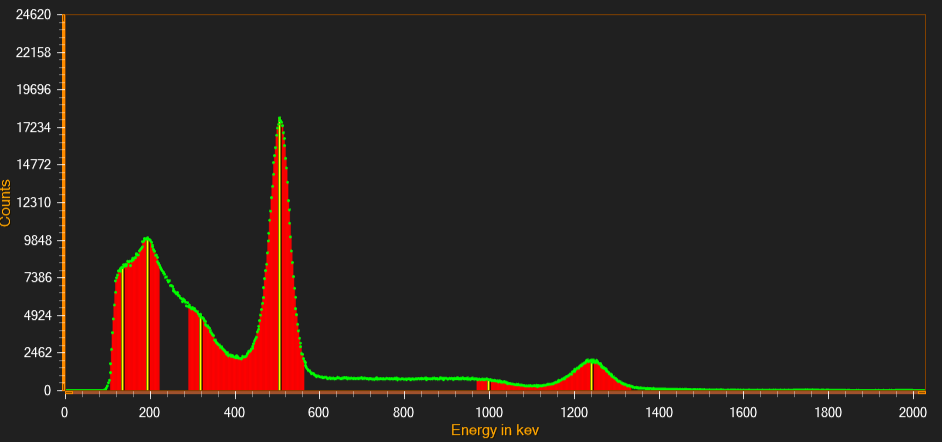
\includegraphics[width = 8 cm]{Figures/Unknown(Na)_spectrum.PNG}
    \caption{Energy plot of unknown source}
    \label{fig:my_label}
\end{figure}
\begin{figure}
    \centering
    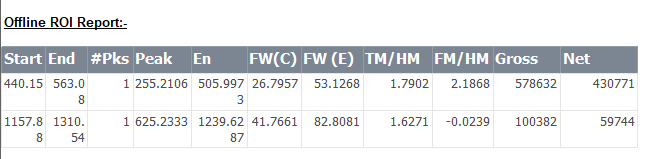
\includegraphics[scale = 0.3]{Figures/Unknown(Na)_report.PNG}
    \caption{Report generated for unknown source}
    \label{fig:my_label}
\end{figure}
We observe a peak energy value at channel number 245.188 with corresponding energy of 511.9069 keV. Considering the characteristic spectrum of Cs-137 for energy Vs channel number; we can conclude that the source might be of Na-22 as the peak is near the value of 511 keV.

\subsection{Mass Absorbption Coefficient for Aluminium}
As per the equation mentioned in the theory section, the intensity of radiation will decrease as it passes through an absorber (in this case - Aluminium). We define a quantity Half Thickness Value (HLV) as the density thickness of the absorbing material that reduces the incident intensity in half. First we obtain the counts without absorber and in subsequent readings we add an absorber slab and take observations.\\
Observations are tabulated below:
% Please add the following required packages to your document preamble:
% \usepackage{longtable}
% Note: It may be necessary to compile the document several times to get a multi-page table to line up properly
\begin{longtable}[c]{|lll|}
\hline
\multicolumn{3}{|c|}{\textbf{Slabs   (Cs-137)}} \\ \hline
\endfirsthead
%
\endhead
%
\multicolumn{1}{|l|}{S. No} & \multicolumn{1}{l|}{Thickness (mm)} & Peak Counts \\ \hline
\multicolumn{1}{|l|}{0} & \multicolumn{1}{l|}{0} & 48299 \\ \hline
\multicolumn{1}{|l|}{1} & \multicolumn{1}{l|}{5} & 41420 \\ \hline
\multicolumn{1}{|l|}{2} & \multicolumn{1}{l|}{10} & 36819 \\ \hline
\multicolumn{1}{|l|}{3} & \multicolumn{1}{l|}{15} & 32860 \\ \hline
\multicolumn{1}{|l|}{4} & \multicolumn{1}{l|}{20} & 29704 \\ \hline
\multicolumn{1}{|l|}{5} & \multicolumn{1}{l|}{25} & 26778 \\ \hline
\multicolumn{1}{|l|}{6} & \multicolumn{1}{l|}{30} & 24288 \\ \hline
\multicolumn{1}{|l|}{7} & \multicolumn{1}{l|}{35} & 21507 \\ \hline
\multicolumn{1}{|l|}{8} & \multicolumn{1}{l|}{40} & 19565 \\ \hline
\multicolumn{1}{|l|}{9} & \multicolumn{1}{l|}{45} & 17193 \\ \hline
\end{longtable}
The plot of how absorber affects the counts is shown in the following plot:
\begin{figure}[H]
    \centering
    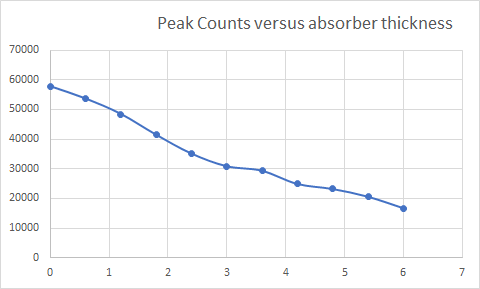
\includegraphics[width = 8 cm]{Figures/absorber.png}
    \caption{Peak Counts Vs Absorber Thickness}
    \label{fig:my_label}
\end{figure}
As we can see from the table as well as the graph above; the counts become half when six slabs are placed together or at the absorber thickness of 30 mm. Hence, HLV in our case is 3 cm. \\
Since density of Al = 2.71 gm/cm$^3$,\\
Density thickness = 2.71 $\times$ 3 = 8.13 gm/cm$^2$,\\
Mass absorption coefficient, m = $\frac{0.693}{8.13}$ = 0.0852 cm$^2$/gm.
    


\section{Results and Discussion}
\begin{itemize}
    \item In SCA, the Scintillation detector's best operating voltage was found to be 553 V (FWHM was 0.28 V and resolution was 9.334 $\%$) when calibrated using Cs-137.
    \item In MCA, the resolution for Cs-137 source came out to be 9.347 $\%$.
    \item The resolution for Co-60 source was found to be 9.347 $\%$.
    \item In the case of mixed sources, four different peaks were obtained (2 peaks from C0-60 while one from each Ba-133 and Cs-137).
    \item The linearity plot had a slope of 2.0878 which is also the energy that one channel corresponds to, in our experiment. Therefore we can safely say that the peak channel of gamma rays is proportional to the energy of gamma energy.
    \item In the case of unknown source, the spectra so obtained gave a peak very close to 511 keV and hence we could conclude that the unknown source is Na-22.
    \item The mass coefficient for aluminium was calculated to be 0.0852 cm$^2$/gm which is near to the literature value of 0.079 cm$^2$/gm.
    \item All the parts of experiment were succesfully conducted and gave satisfactory results.
\end{itemize}
\end{document}





\end{document}
%
% ****** End of file apssamp.tex ******
